\section{Methods}
\label{sec:methods}

The proposed system for identifying and evaluating the fatigue indicators is summarized in Figure \ref{prepost_system}. The following sections will provide in-depth explanations for each part of the system. %As a summary, all the subjects were equipped with body-mounted IMUs and performed a specific SET adjusted to their discipline. Data was collected from in-hand walking and trotting before SET (pre-SET) and after SET (post-SET), and subsequently, the signals from IMUs were preprocessed and windowed based on strides. Biomechanical features were extracted from the windows. For this study, the performance state of horses during pre-SET measurements was assigned as "non-fatigue," while for the post-SET, it was considered "fatigue". A Neighborhood Component Analysis (NCA) was applied to the extracted features to identify the important fatigue indicators. Finally, to quantify the importance of the selected features, they were implemented in classification algorithms, and the performances of the trained classification models were compared and analyzed. The sequence of tasks during SET is demonstrated in Fig \ref{SET}.

\begin{figure}[htbp]
\centering
\includegraphics[width=.95\linewidth]{chapters/prepost/figures/Untitled_HQ.png}
\caption{Our used method for identification and evaluation of fatigue indicators.}
\label{prepost_system}
\end{figure}

\begin{figure}[htbp]
\centering
\includegraphics[width=.95\linewidth]{chapters/prepost/figures/SET.png}
\caption{Order of the tasks for horses to perform a \gls{set}.}
\label{SET}
\end{figure}

\subsection{Data preparation}
%\subsection{Participants}

The data were collected from the horses that were introduced in Chapter \ref{chapter:data}. They were sixty horses, consisting of sixteen young Friesian stallions, twenty-eight international eventing horses, ten elite showjumping, and six elite dressage horses. The average age of all the horses was 9.6 $\pm$ 4.5 years, while for Friesian horses, eventing, showjumping, and dressage horses were 3.2 $\pm$ 0.4, 11.1 $\pm$ 3.0, 12.7 $\pm$ 1.6, and 13.8 $\pm$ 1.9 years, respectively. 

All the horses other than the Friesian horses were competing under \gls{fei} rules. The elite dressage and showjumping horses were competing at Grand Prix level and were all qualified for the Olympic games in Tokyo 2020. Moreover, six eventing horses were also qualified for these Olympic games, while other eventing horses were competing at the international level (from Concours Complet International 2-star (CCI2*) to 5-star (CCI5*).

All the participants were examined for lameness pre-\gls{set} and post-\gls{set} by a veterinarian. The ones that presented lameness during the examinations were excluded from this chapter. Animal Ethics Committee of Utrecht University gave the ethical permissions for the measurement of young Friesian horses. The Committee concluded that ethical approval was not needed for measuring the remaining horses since it did not qualify as an animal experiment under The Netherlands law.

%\subsection{Data collection}

The data in this chapter was collected from the horses while walking and trotting in-hand before \gls{set} (pre-\gls{set}) and after \gls{set} (post-\gls{set}). The assigned \gls{set} for each horse was different based on the discipline. For Friesian and eventing horses, we performed the \gls{set} protocols described in previous studies \cite{MUNSTERS2013193} and \cite{CBM}. The \gls{set} protocol for the showjumping horses was adapted from two studies \cite{Munk2013EffectsJumping,articlesoares}. For dressage horses, the same Friesian horses \gls{set} protocol was used with an addition of an adapted Grand Prix test  \cite{FEI_test}.

During the measurement, the horses were equipped with seven ProMove-mini \gls{imu}s \cite{456} attached to the sacrum, withers, head (poll), and the lateral aspect of all four limbs (cannon bone). The \gls{imu}s contained a tri-axial accelerometer and a tri-axial gyroscope and were set to a sampling rate of 200 Hz, acceleration range of ±16 g, and angular velocity range of ±2000 deg/s. Figure \ref{fig:IMUplacement} demonstrates the \gls{imu} locations and orientations on the horse body. 

In addition to the biomechanics measurements, \gls{lac} was also measured. Blood samples were extracted from the jugular vein of horses once before pre-\gls{set}, three to four times during the \gls{set}, and once before post-\gls{set}, which the latter was immediately after the cool-down period as indicated by the recovery \gls{lac} in Figure \ref{SET}. Following each collection, the collected blood sample was inserted into a portable hand-held measurement device (Lactate Pro2, Arkray Inc., Kyoto, Japan) for instant plasma \gls{lac} calculation.  
 

\begin{figure}[htbp]
\centering
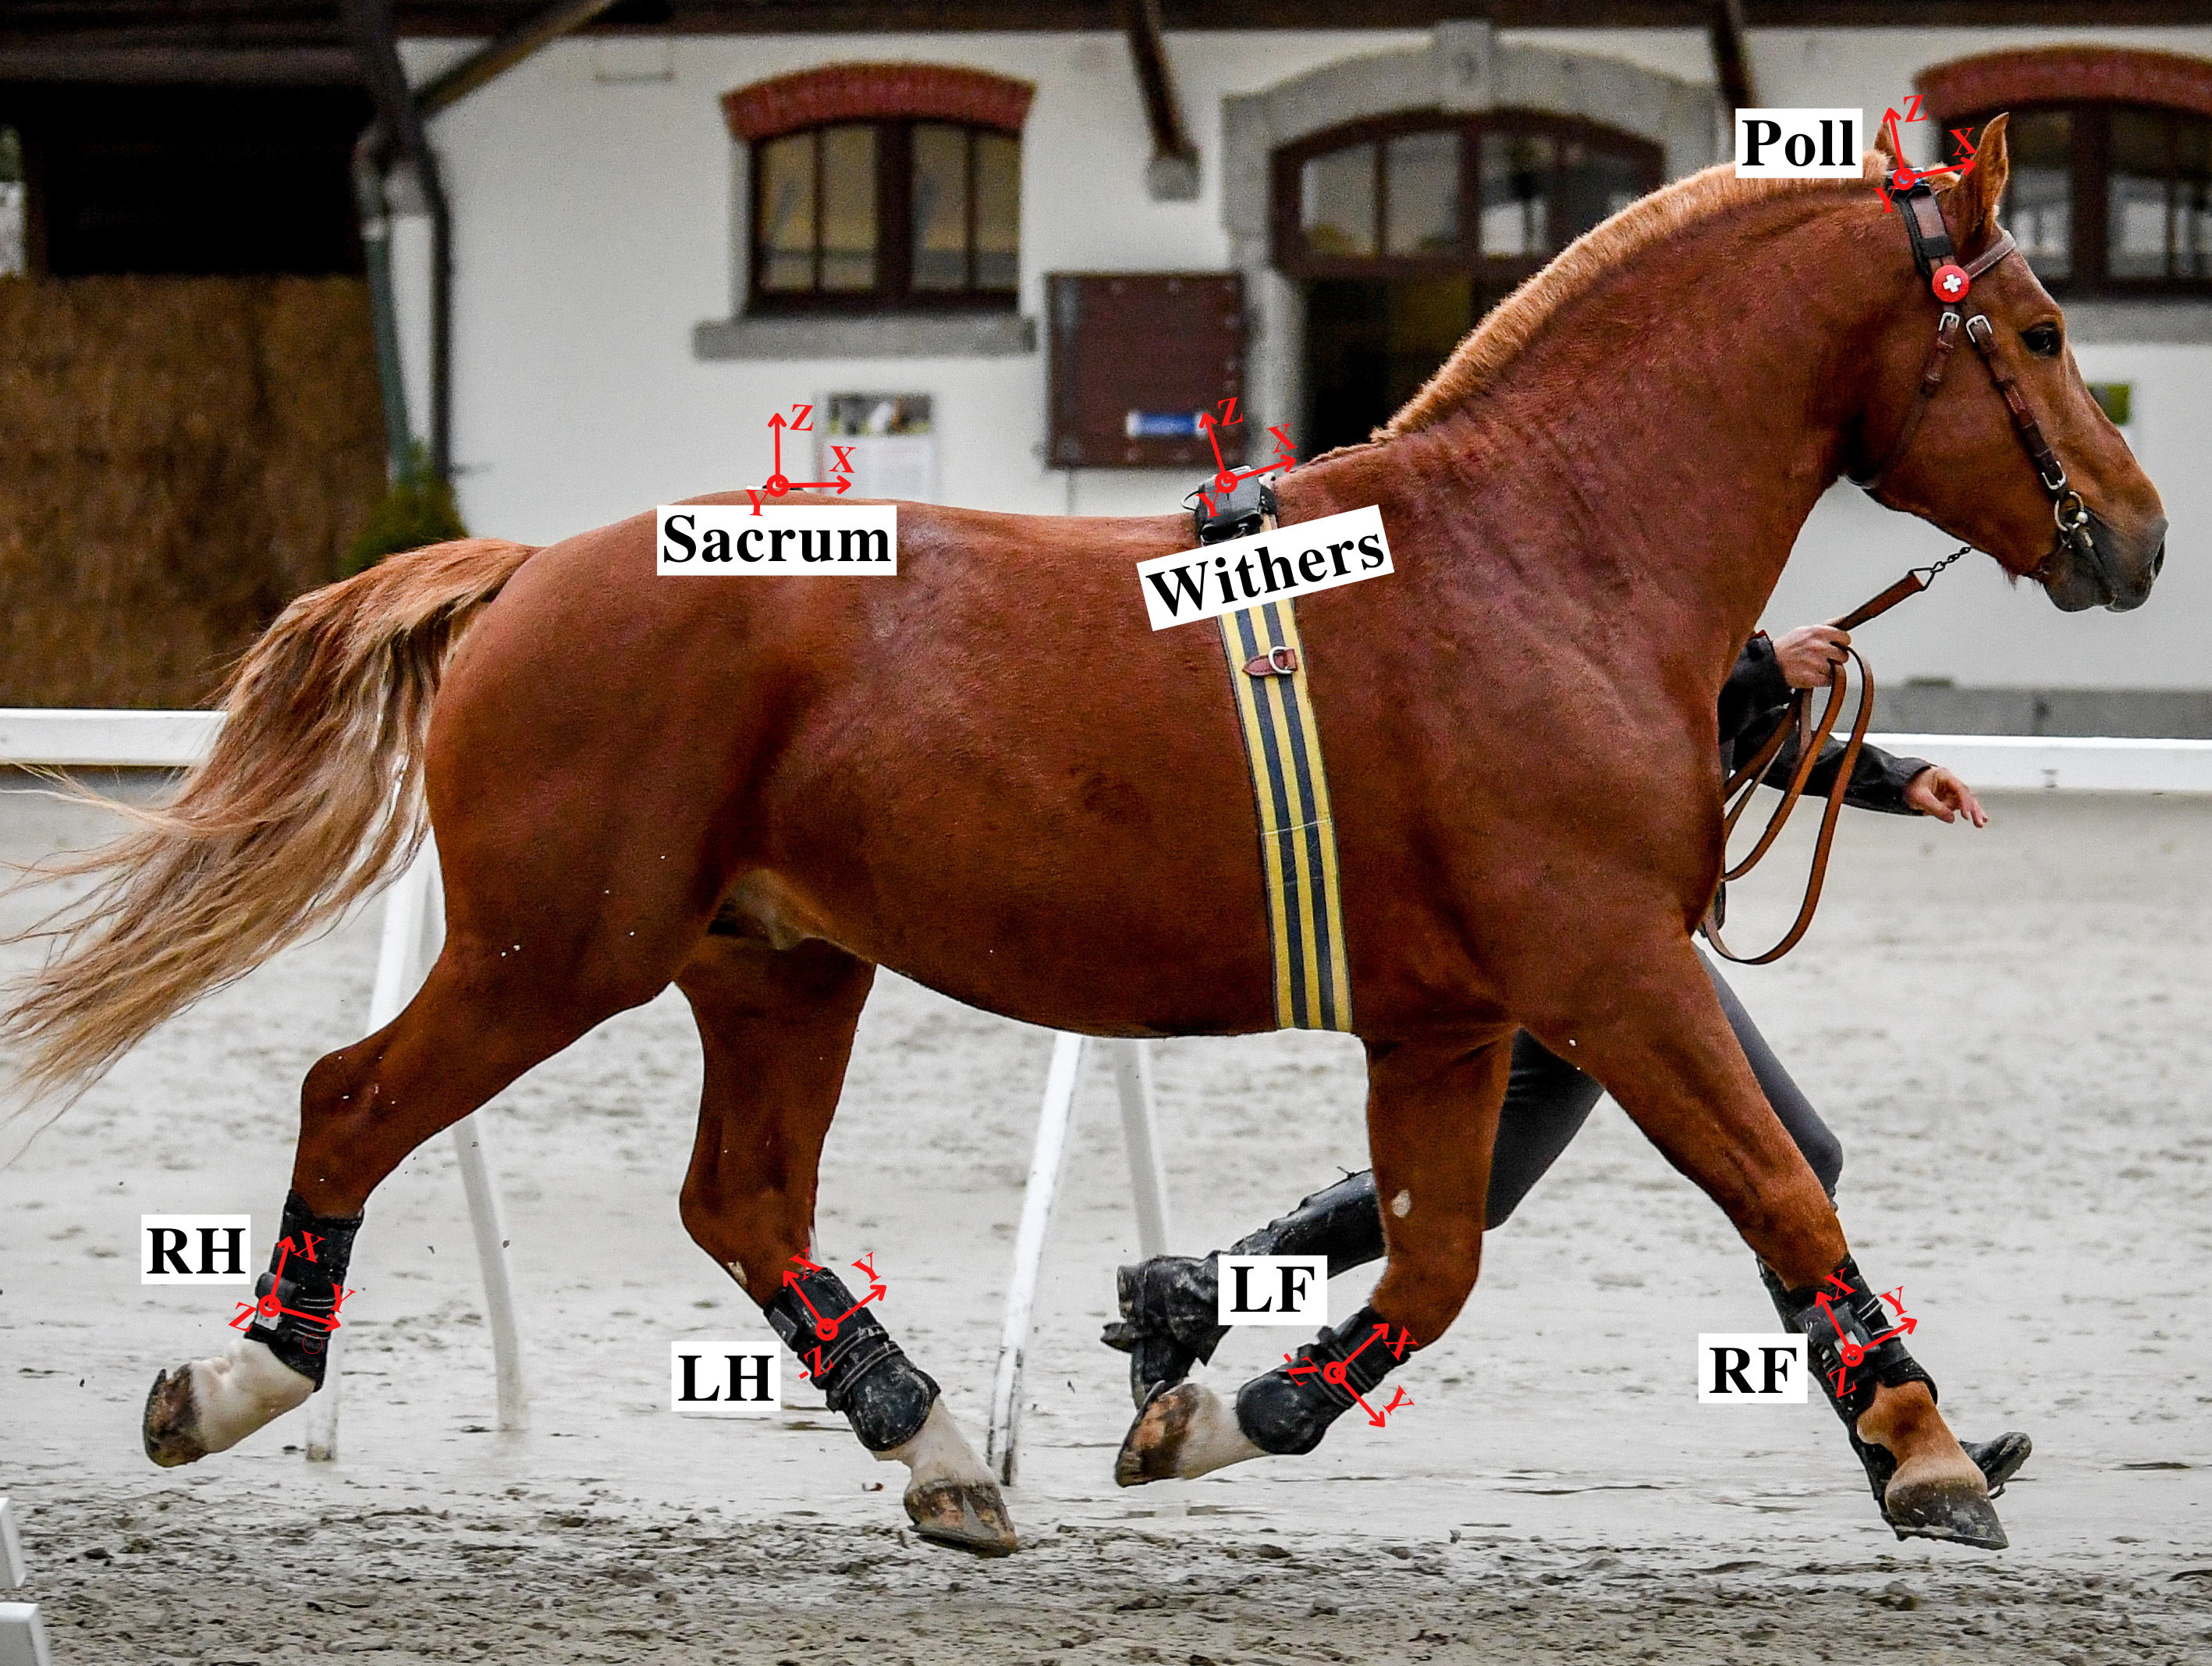
\includegraphics[width=.95\linewidth]{chapters/prepost/figures/Sacrum_HQ.png}
\caption{IMUs locations and orientations on horse body.}
\label{fig:IMUplacement}
\end{figure}

As demonstrated in Fig \ref{fig:IMUplacement}, the three axes of rotation for the sacrum, withers, and poll \gls{imu}s were x,y, and z, which were defined in the order as roll, pitch, and yaw angles. For the limbs, x, y, and z-axis were internal/external rotation, retraction/protraction, and abduction/adduction axis, respectively \cite{456}. Furthermore, the three axes of horse's locomotion, in general, were the longitudinal axis (aligned to the forward locomotion and parallel to the ground), the vertical axis (perpendicular to the ground or parallel to the gravitational force vector), and the mediolateral axis (perpendicular to longitudinal and vertical axes).

%\subsection{Datasets and subsets}

Based on the maximum \gls{lac} values during \gls{set}, the relative intensity level of \gls{set} can be determined. Therefore, as presented in Table \ref{lactate}, the lactate values were used to generate three datasets. The three datasets were: 

\begin{itemize}
\item Dataset 1: Horses performed in both high intensity and low intensity \gls{set}s (all the participants)
\item Dataset 2: Horses performed in high intensity \gls{set} only, which were eventing and young Friesian horses
\item Dataset 3: Horses performed in low intensity \gls{set} only, which were showjumping and dressage horses
\end{itemize} 

 \begin{table}[!htbp] 
    \centering
      \caption{Number, age (in years), and plasma lactate concentration (post-SET and the maximum value during SET) of horses by datasets}% Add 'table' caption

    
    \resizebox{\linewidth}{!}{% 
    \begin{tabular}{lcccccc}
    
   && & \multicolumn{4}{c}{\bf Plasma lactate concentration (mmol/l)}\\
    
    \cmidrule{4-7}
    
 & & &  \multicolumn{2}{c}{\bf Maximum} & \multicolumn{2}{c}{\bf Recovery} \\   

\cmidrule{4-5} \cmidrule{6-7}

\multicolumn{1}{c}{\bf Dataset}  & \multicolumn{1}{c}{\bf Number} & \multicolumn{1}{c}{\bf Age (Mean ± SD)} &  \multicolumn{1}{c}{\bf Mean (SD)} & \multicolumn{1}{c}{\bf Range} &  \multicolumn{1}{c}{\bf Mean (SD)} & \multicolumn{1}{c}{\bf Range} \\   

\midrule

\multicolumn{1}{l}{Dataset 1} & 60 & 9.6 ± 4.5 & \multicolumn{1}{c}{3.49 (1.90)} & \multicolumn{1}{c}{0.90 - 10.00} & \multicolumn{1}{c}{1.23 (0.55)} & \multicolumn{1}{c}{0.60 - 4.00} \\ [0.4 em] 

\multicolumn{1}{l}{Dataset 2}  & 44 & 8.3 ± 4.5 & \multicolumn{1}{c}{4.04 (1.80)} & \multicolumn{1}{c}{1.60 - 10.00} & \multicolumn{1}{c}{1.29 (0.57)} & \multicolumn{1}{c}{0.70 - 4.00} \\ [0.4 em]    

\multicolumn{1}{l}{Dataset 3}  & 16 & 13.1 ± 1.8 & \multicolumn{1}{c}{1.62 (0.57)} & \multicolumn{1}{c}{0.90 - 2.90} & \multicolumn{1}{c}{0.98 (0.40)} & \multicolumn{1}{c}{0.60 - 2.40} \\ [0.4 em]

       \bottomrule
    \end{tabular}}
        
    \label{lactate}
    \end{table}

The \gls{lac} of all participants pre-\gls{set} was considered low and can be indicated as normal resting values (between 0.6 and 0.8 \gls{mmol/L}). Dataset 1 consisted of all horses, while datasets 2 and 3 were based on the disciplines or breeds that performed in higher and lower \gls{set} intensity levels, respectively. 

The \gls{set} intensity levels were defined using the maximum \gls{lac} values as presented in Table \ref{lactate}, where the average for dataset 2 was more than 4.00 \gls{mmol/L}, while the average for dataset 3 was less than 1.70 \gls{mmol/L}. We calculated the average values and deviations of the datasets to serve as the intensity indicators for the \gls{set}. Consequently, we designated the intensities of dataset 2 and dataset 3 as high and low, respectively.

It should be mentioned that for simplicity in comparing to levels of \gls{set}, we considered the \gls{set}s of eventers and young Friesian horses as "high" intensity. In exercise physiology, these \gls{set}s are submaximal \gls{set}s with moderate \gls{lac} values and not defined as high-intensity levels, like maximal exercise test reaching maximal \gls{lac} levels. According to the equine physiology literature, a high-intensity level \gls{set} can induce \gls{lac} values as high as 32 \gls{mmol/L} \cite{patrichttps://doi.org/10.1111/j.2042-3306.1988.tb01470.x}. In general, Warmblood sport horses (including all the horses in this study) will almost not reach these high levels of \gls{lac} as the nature of their disciplines is submaximal. Thus, \gls{lac} higher than 4 \gls{mmol/L} is considered as high intensity for Warmblood horses. There were \gls{lac} value differences between \gls{set}s of different disciplines in this study, hence, we assigned the "high" intensity label to the \gls{set} of disciplines with higher \gls{lac} values and "low" to those with lower \gls{lac} values.
 
 As shown in Figure \ref{prepost_system}, we derived three subsets from each dataset, which comprised data from walking, trotting, and both walking and trotting. The latter subset is referred to as "Walk+Trot" in this chapter. This step was taken since our goal was to focus on the important indicator of each gait as well as investigate fatigue indicators independent of gait type in the Walk+Trot subsets. Feature extraction, feature normalization, feature selection, and model development and evaluation, were taken on all of the nine subsets. 

%\subsection{Data preprocessing}

The raw signals derived from the \gls{imu}s (three signals of acceleration and three signals of angular velocity) were low-pass filtered (fourth-order Butterworth filter and 30 Hz cut-off frequency) for noise reduction \cite{456}. Then, the filtered signals were windowed into strides (from hoof-on to next hoof-on of the right front limb) by implementing the estimation method from Chapter \ref{chapter:Step} on the raw signals that were extracted from the \gls{imu} mounted on right front limb. The pre-\gls{set} and post-\gls{set} data were separated from the start, hence, the strides were labeled as pre-\gls{set} or post-\gls{set} without performing an exhaustive labeling process. 

\subsection{Feature extraction}

As shown in Table \ref{deff}, fifty-two features were calculated per stride, which were:

\begin{itemize} 

\item \textbf{Gait events} (stride, stance, and swing duration) were determined using the estimated hoof-on/off moments from Chapter \ref{chapter:Step} estimation model.

\item \textbf{Speed} was estimated using the speed estimation model from Chapter \ref{chapter:Speed}, which receives acceleration and angular velocity signals from the sacrum and limb \gls{imu}s and accurately estimates the speed. 

\item \textbf{Angular range of motion of the limbs} around their three axes, which were protraction/ retraction, adduction/abduction, and internal/external rotation, were calculated by considering the limb as cannon bone, carpal joint as the reference point, and axes as demonstrated in Figure \ref{fig:IMUplacement}. 

\item \textbf{Angular range of motion of the head, pelvis, and withers} around the three axes, namely roll, yaw, and pitch, were determined by considering the reference point as the center of the \gls{imu}s and axes as depicted in Figure \ref{fig:IMUplacement}. The angular ranges of motions were calculated by integrating the angular velocity signals from \gls{imu}s. 

\item \textbf{MaxDiff, MinDiff, and displacement range of motions}: To calculate the displacement features, we applied a cyclical integration process on acceleration signals, described in \cite{Pfau2013}. MaxDiff and MinDiff are essential indicators of movement (a)symmetry and were calculated using the difference between the two peaks (MaxDiff) and troughs (MinDiff) of the sacrum, withers, and head vertical (z-axis) displacement of a stride \cite{Kramer2004}. Also, the longitudinal, mediolateral, and vertical displacement range of motion of the sacrum, withers, head, and limbs of each stride were determined. 
\end{itemize} 


 \begin{table}[!htbp] 
    \centering
      \caption{Extracted Features from strides}% Add 'table' caption

    
    \resizebox{\linewidth}{!}{% 
    \begin{tabular}{llc}
    
   \toprule
    
    Feature name & Extracted from IMU mounted on & Number\\
    
\midrule

\multicolumn{1}{l}{Stride, stance, and swing duration} & \multicolumn{1}{l}{Right front limb} & 3 \\ [0.4 em]   

\multicolumn{1}{l}{Speed} & \multicolumn{1}{l}{Sacrum, Right front limb} & 1 \\[0.4 em]

\multicolumn{1}{l}{MaxDiff and MinDiff} & \multicolumn{1}{l}{Sacrum, Withers, Head}& 6  \\[0.4 em]

\multicolumn{1}{l}{Protraction/retraction range of motion} & \multicolumn{1}{l}{Limbs} & 4 \\[0.4 em]

\multicolumn{1}{l}{Adduction/abduction range of motion} & \multicolumn{1}{l}{Limbs} & 4 \\[0.4 em]

\multicolumn{1}{l}{Internal/external rotation range of motion} & \multicolumn{1}{l}{Limbs} & 4 \\[0.4 em]

\multicolumn{1}{l}{Roll angle range of motion} & \multicolumn{1}{l}{Sacrum, Withers, Head} & 3 \\[0.4 em]

\multicolumn{1}{l}{Pitch angle range of motion} & \multicolumn{1}{l}{Sacrum, Withers, Head} & 3 \\[0.4 em]

\multicolumn{1}{l}{Yaw angle range of motion} & \multicolumn{1}{l}{Sacrum, Withers, Head} & 3 \\[0.4 em]

\multicolumn{1}{l}{Longitudinal displacement} & \multicolumn{1}{l}{Sacrum, Withers, Head, Limbs} & 7 \\[0 em]

\multicolumn{1}{l}{(Along horse longitudinal axis)} &  &  \\[0.4 em]

\multicolumn{1}{l}{Mediolateral displacement} & \multicolumn{1}{l}{Sacrum, Withers, Head, Limbs} & 7 \\[0 em]

\multicolumn{1}{l}{(Along horse mediolateral axis)} & &  \\[0.4 em]

\multicolumn{1}{l}{Vertical displacement (horse vertical axis)} & \multicolumn{1}{l}{Sacrum, Withers, Head, Limbs} & 7 \\[0.1 em]


\midrule

\multicolumn{1}{l}{Total} & & 52  \\[0.1 em]

\bottomrule
\end{tabular}}
        
    \label{deff}

    \end{table}
    

%\subsection{Feature normalization}

We combined the features from pre-\gls{set} and post-\gls{set} for each participant and subsequently normalized them within the range of 0 to 1. The intra-individual normalization allows us to emphasize the distinctions between pre-\gls{set} and post-\gls{set} measurements, rather than being influenced by inter-individual variations, which can be influenced by numerous factors, including physical fitness levels. 

We opted to assign a representative of each feature for each horse in each trial (pre-\gls{set} or post-\gls{set}) rather than analyzing the strides of each horse individually. This approach allows us to focus on the overall pre-\gls{set} and post-\gls{set} variations, rather than the differences in individual strides. We considered the mean and variability values of the extracted features as the most appropriate representatives of the variations. In terms of its definition, variability specifies the dispersion of data points and serves as a statistical summary of these data points. In other words, it can be used as a metric to assess whether a horse's strides exhibit consistency during pre- or post-\gls{set} \cite{wight,Nauwelaerts}.  Each feature's mean and variability were calculated for each horse during both trials (pre-\gls{set} or post-\gls{set}), which resulted in 104 features for each horse during each trial. 

To determine the most suitable variability metrics, four metrics were selected based on the literature, namely root mean square, coefficient of variation, standard deviation, and variance \cite{Nauwelaerts,wight,burdack,ESTEP2018111,s21144792}. These metrics were then evaluated on each subset, as illustrated in the "Third Loop" of Figure \ref{prepost_system}. The best variability metric was selected based on the classification model performance results for each subset as indicated by the output of the "Third Loop" feeding into the "Second Loop" in Figure \ref{prepost_system}.

%\subsection{Feature selection}

The seven body-mounted \gls{imu}s were required to extract the 104 features for the model. However, equipping a horse with seven \gls{imu}s can be cumbersome in practice. The number of features can be reduced by selecting only the meaningful ones, potentially leading to a reduction in the number of \gls{imu}s required for extracting the chosen features. Selecting important features offers additional advantages, such as preventing the model from overfitting and enhancing overall accuracy. Hence, we applied a \gls{nca} \cite{10.5555/2976040.2976105} to the features within each subset. \gls{nca} assigns a weight to each feature, and based on these assigned weights, the features within each subset were ranked. 

It's important to note that the durations of speed and gait events were calculated without regard to the selection or rejection by the proposed feature selection model. The comparison of these features between the pre-\gls{set} and post-\gls{set} was conducted separately. These features were selected for additional comparison owing to their significance in the literature on equine fatigue, as referenced in the literature \cite{Cottin2006EffectTraining,Colborne2001ElectromyographicStudy.,Williams2018ElectromyographyTechnology, Pugliese2020EffectStudy,parkes_2019_the,Takahashi2021EffectsRaces}.

\subsection{Model training, testing, and optimization}
\label{methodmodel}

According to the feature evaluation step in Figure \ref{prepost_system}, the importance of selected features per subset (walk, trot, or Walk+Trot) was quantified by testing the performance of classification models that trained solely on those features. The purpose of classification models was to classify an input stride to pre/post-\gls{set} (or non-fatigue/fatigue). We trained a classification model using the first selected feature by \gls{nca} as the feature for each subset and then evaluated the model performance. In the following steps, we added the next-ranked (second-ranked to nth-ranked) feature selected by \gls{nca} and evaluated the model performance that was trained by the selected feature in each step and the higher-ranked features. The feature addition process was terminated as soon as the accuracy of the classification model decreased, and then, constituent features of the model with the highest accuracy were reported as the most significant fatigue indicators for that subset. 

In terms of choosing the best performing algorithm, four machine learning algorithms were implemented as the model training and testing method in the "Fourth Loop" of Figure \ref{prepost_system}. The tested algorithms were \gls{svm}, \gls{knn}, decision tree, Naive Bayes, and logistic regression.

As shown in Figure \ref{prepost_system}, for each subset, the features were selected using leave-one-subject-out \cite{articlevarma} to prevent biased results in the "Fourth Loop" of the system (Figure \ref{prepost_system}. We also implemented leave-one-subject-out on the classification models training to be certain that a participant has been used at least one time as training and testing data \cite{darbandi_2021_using}. 

The performances of models were quantified by calculating the performance metrics (using true positive, false positive, true negative, and false negative) as follows: 

\begin{itemize}
  \item True positive (TP): The number of predictions if the true class is pre-\gls{set} and the prediction is pre-\gls{set}
    
  \item False positive (FP): The number of predictions if the true class is post-\gls{set} and the prediction is pre-\gls{set}
  
    \item True negative (TN): The number of predictions if the true class is post-\gls{set} and the prediction is post-\gls{set}
  
      \item False negative (FN): The number of predictions if the true class is pre-\gls{set} and the prediction is post-\gls{set}
  
      \item Accuracy = $\dfrac{TP + TN}{TP + FP + TN + FN}$
  
      \item Sensitivity or classification accuracy of pre-\gls{set} strides = $\dfrac{TP}{TP + FN}$
  
      \item Specificity or classification accuracy of post-\gls{set} strides = $\dfrac{TN}{TN + FP}$
  \end{itemize}


 The selected features and the performance results of the models per subset are compared in the next section. Matlab R2020a (MathWorks Inc., Natick, MA, USA) was used for all the computations in this chapter. 